\documentclass[twocolumn,a4paper,10pt,review,5p]{elsarticle}

\usepackage{amsmath}
\usepackage{lineno,hyperref}
\usepackage{tabularx}
\usepackage{amssymb}
\usepackage{booktabs}
\modulolinenumbers[5]

\journal{Journal of Web Semantics}

%% `Elsevier LaTeX' style
\bibliographystyle{elsarticle-num}

%%%%%%%%%%%%%%%%%%%%%%%

\begin{document}

% =========================================
% front matter

\begin{frontmatter}

\title{Adversarial Ranking for Knowledge Graph Representation with Bagging}

% ----------------------
% affiliations

\author[hrbaddress]{Qingsong Meng}

\author[ucasaddress,hrbaddress]{Xiang Zhang}
\ead{xiang.zhang@nlpr.ia.ac.cn} % `ead' stands for email address

\author[ucasaddress]{Shizhu He}
\ead{shizhu.he@nlpr.ia.ac.cn}

\author[ucasaddress]{Jun Zhao\corref{correspondingauthor}}
\ead{jzhao@nlpr.ia.ac.cn}

\cortext[correspondingauthor]{Corresponding author}
\address[hrbaddress]{Harbin University of Science and Technology, No.52 Xuefu Road, Nangang District, Harbin, 150080, China}
\address[ucasaddress]{University of Chinese Academy of Sciences, No.19(A) Yuquan Road, Shijingshan District, Beijing, P.R.China 100049}

% -------------------------
% abstract + keywords

\begin{abstract}
Adversarially training.
\end{abstract}

\begin{keyword}
Knowledge Graph \sep{} Representation Learning \sep{} Adversarial Training \sep{} Bagging
\MSC[2010] 68T30 \sep{} 68T50
\end{keyword}

\end{frontmatter}

% ==========================================
% main text

\linenumbers{}

% ------------------------
% introduction

\section{Introduction}
\label{sec:intro}

Knowledge graph is an important component in many natural language processing applications nowadays, such as natural language inference, question answering, and task-oriented dialogue generation. One of the fundamental tasks in the field is \emph{representation learning}, which aims to learn a representation for each \emph{entity} and \emph{relation} in a knowledge graph. Consider the following example. The triple \emph{(Leonhard Euler, BornIn, Basel)} is a selected fact from a typical knowledge graph, \emph{WikiData}\footnote{https://www.wikidata.org/}. Representation learning models assign a vectorized representation respectively to the head entity \emph{Leonhard Euler} and the tail entity \emph{Basel}, and some models also give a representation for each relation, namely \emph{BornIn} in this example. In general, there must be some characteristics to hold or constraints to meet for these representations, which facilitate other tasks like inference or completion on the knowledge graph.

% TODO: avoid using formula but to use graphs instead in introduction

One of the most popular constraints is the translation assumption. Borders et al.~\cite{TransE2013} first proposed the \emph{TransE} model, in which the representation of a tail entity~$(t)$ could be arithmetically computed by adding the representations of the corresponding head entity~$(h)$ and relation~$(r)$, that is, $h + r \simeq t$. This gives a very concise and beautiful geometric explanation that every relation can move or \emph{translate} an entity embedding into another, and hence its name \emph{TransE}. Specifically, they try to minimize a hinge loss with a predefined margin as follows,
\[
    \min\sum_{\substack{(h, r, t)\in S,\\ (h^\prime, r, t^\prime)\in S^\prime }}
        {\left[\gamma + f(h, r, t) - f(h^\prime, r, t^\prime)\right]}_+,
\]
where $S$ is the set of triples and $S'$ is the set of negative samples. $f(h, r, t)$ can be viewed as an energy or scoring function which in their case is an L1 or L2 norm of $h + r - t$.

The training method above shares the same basic framework with many other work. For instance, \emph{TransR}~\cite{TransR2015} introduces a mapping from the entity space to the relation space, where the scoring functions is $\lVert h M_r + r - t M_r \rVert_2^2 $, and \emph{Neural Tensor Network} (NTN)~\cite{NTN} utilizes a bilinear model and a single layer neural network to achieve impressive results, whose scoring function is $u_r^T \tanh(h^T W_r^{[1:k]}t + V_r[h;t] + b_r)$. The training framework can be viewed as a discriminative model because the key scoring function aims to predict high scores for real possible facts in a knowledge graph while lowers the scores for the sampled negative facts, thus we may expect it to give a reasonable high score for some missing but possible facts at testing time.

Despite the success of these discriminative models, there are two challenges remaining for the problem.
The first challenge is the improperness of negative sampling, which can be either completely absurd or indeed authentic because of the random-choosing strategy.
The model can differentiate them with little effort for the absurd samples while the authentic negative samples will mislead the model to a wrong direction. For example, there are two facts in WikiData \emph{(Leonhard Euler, child, Chistoph Euler)} and \emph{(Leonhard Euler, child, Johann Euler)}, where the two different entities share the same head entity, namely a one-to-many relation. To construct a negative sample, we may simply substituting the tail entity by another absurd entity, say, \emph{Basel}, which yields a triple \emph{(Leonhard Euler, child, Basel)}. The model will receive no improvement because the entity is even a city rather than a person. But if an either child is selected to act as the tail entity for the other triple which further serves as a negative sample, the model will probably get fooled.

\begin{table}
    \centering
    \begin{tabular}{ccc}
        \toprule
        percentiles & FB15k & WN18 \\
        \midrule
        25\% &  1   & 1  \\
        50\% &  1   & 1 \\
        75\% &  2   & 1 \\
        90\% &  5   & 2 \\
        99\% &  28  & 10 \\
        max & 3590  &  471 \\
        \midrule
        mean &  3.14 & 1.65 \\
        count & 153630 & 85532 \\
        standard deviation & 18.36 & 5.08 \\
        \bottomrule
    \end{tabular}
    \caption{Statistics of tail entities given the same head entity and relation pair in the training data. Both the FB15k and WN18 dataset have a much greater mean than 1. At least 25\% of FB15k (and 10\% of WN18) distinct pairs of head entity and relation have more than 1 tail entity, which shows the ubiquitous presence of one-to-many relations. }
\label{one-to-many}
\end{table}

% TODO: directly talk about the challenge, summarize it rather than explain it

The second challenge is the more or less subtle. Discrmininative models can give a score to every single new triple, but lacks the ability to predict the entity probablistic distribution in a global view. Since the training data is always incomplete and the true data distribution is unknown, it might be a hard decision for a discrminative model to make that whether a fact is just missing or actually impossible to appear. Things might get even worse due to the ubiquitous presence of the one-to-many relations, as proven by the statistics in Table~\ref{one-to-many}. To overcome the difficulty, many previous work designed delicate neural models~\cite{NTN} and trans-* series models~\cite{TransH2014,TransR2015} to enhance the performance. It's no doubt difficult to design an even more perfect discriminative model. Xiao et al.~\cite{TransG} novelly proposed \emph{TransG} as a generative model to deal with the multi-semantic phenomenon in many one-to-many relations. While it still requires the traslation assumption to hold, TransG inspires us to adopt the generative approach along with its theoritical framework and ability to incorporate complex prior.

Taking the above challenges into consideration, we systematically propose an adversarial training method to learn a discriminator and a generator in the meantime. The generator could predict the probability distribution, while the discriminator would still function as previous models.

At the generator side, we discard the translation assumption. For simplicity, we just assume the head and relation are both uniformly distributed, thus concentrate on directly modeling the conditional probability $p(t\mid h, r)$ and generate the tail entity given its head and relation. As the generator is getting better, it would predict better entities as negative samples which is more useful for the discriminator than those randomly chosen ones, thus cures the problem of absurd negative sample.

At the discriminator side, inspired by the idea from IRGAN~\cite{IRGAN}, we build a ranking-based loss which will not take generated samples as complete negative samples but only give them lower rank compared to the positive sample.

We have stated the effects of the discriminative and generative models in this task. We have to note that the generator can do much more than generating negative samples, it has indeed the power to prediction as well as the discrminator. Empirically we know neither model could completely beat the opposite. The characteristics of these two are quite different and we thus have two very heterogeneous models in the adversarial training setting, which happens to meet the requirement for ensemble learning. Therefore we adopt a simple bagging method between the two only models and receive very impressive results.

Our contributions are thus two-fold:
\begin{itemize}
    \item We propose an adversarial ranking training for representation learning of knowledge graph, in order to generate better negative samples and make better use of them.
    \item To exploit the power of both the generator and discriminator, we propose to use a simple bagging method which beats all the baselines and achieves the best result.
\end{itemize}


% ---------------------------------------
% method

\section{Methods}

We formulate our adversarial training setting in this section. As stated in the previous section, our model consists of a discrmininator and a generator, which are adversarially trained and exploited together through a bagging method. We report each components in the following subsections.

\subsection{Notations}

A knowledge graph $\mathcal{K}$ can be defined as a triple $(\mathcal{E}, \mathcal{R}, \mathcal{F})$, where $\mathcal{E}$ is the set of entities, $\mathcal{R}$ is the set of relations, and $\mathcal{F}$ is the set of facts. Every fact $f\in \mathcal{F}$ is again a triple $(h, r, t), \forall h,t\in\mathcal{E}, r\in\mathcal{R}$. The training data $X$ is a subset of the real facts, $X \subset \mathcal{F}$

We defined the discrminator $d$ as a scoring function which maps a triple to a scalar, namely $d: \mathcal{F}\rightarrow \mathbb{R}$. The generator on the contrary tries to maximize the joint probability $p(h, r, t)$ which is in turn proportional to the conditional distribution $p_g(t \mid h, r)$. We thus defined the generator as a function $g: \mathcal{E} \times \mathcal{R} \rightarrow \mathbb{R}^{\lvert \mathcal{E} \rvert}$.

\subsection{Discriminator}

As discussed in the Section~\ref{sec:intro}, we use a ranking-based objective when training the discrminator. Here we defined the score distance as follows,
\[
    sd(\hat t, t^*; h, r) := \lvert d(h, r, t) - d(h, r, t^*) \rvert,
\]
where $h$ and $r$ are the head entity and relation respectively, $t$ is the tail entity from training data, and $t^*$ is a tail entity coming from either the generator or the training data, which making the score distance be 0 in the latter case.

In the following we defined the ranking function,
\begin{align*}
    rank_\tau(t, {\{\tilde t \}}_{i=1}^K)
    &= \frac{\exp(sd(t, t; h, r) / \tau)}
        {\sum_{t^*\in \{t\} \cup {\{\tilde t \}}_{i=1}^K } \exp (sd(t, t^*; h, r) / \tau) } \\
    &= \frac{1}
        {\sum_{t^*\in \{t\} \cup {\{\tilde t \}}_{i=1}^K } \exp (sd(t, t^*; h, r) / \tau) },
\end{align*}
where $t$ is a tail entity from the training data, $\tilde t$ is a tail entity sampled from the generator, $K$ indicates the number of tail entity samples in the ranking list, and $\tau$ is the temperature hyperparameter to control the variance of the softmax function.

We then define the training loss for the discriminator as follows,
\begin{align*}
    \max_d \sum_{(h, r, t)\in X}
        &\mathbb{E}_{\tilde t_1, \dots, \tilde t_K \sim p_g(t \mid h, r)}
            rank_\tau(t, {\{\tilde t \}}_{i=1}^K) \\
        &- \mathbb{E}_{\tilde t \sim p_g(t \mid h, r)}
            rank_\tau(\tilde t, t)
\end{align*}

Note the parameters of the discrminator only occur inside the expectation term. We can just draw samples from the distribution produced by the generator and feed them to the discrminator, and the optimization algorithm will work as it is intended to do. The orange lines in Figure~\ref{system-overview} illustrate the process.

\subsection{Generator}

The generator will output an probabilistic measure of the set of all entities $\mathcal{E}$. We minimize the following cross entropy term defined through the discrminators' feedback,

\begin{align*}
    \min_g \sum_{(h, r, t)\in X}
        \mathbb{E}_{\tilde t \sim p_g(t \mid h, r)}
            \frac{\exp(d(h, r, \tilde t) / \tau)}
                 {\sum_{t^* \in \{ t, \tilde t\}} \exp(d(h, r, t^*) / \tau)}
\end{align*}

However, it's not possible to directly optimize the above loss function using gradient-based algorithms. In practice, we have to sample a discrete distribution, which makes a simple reparemeterization trick~\cite{VAE} fail. A popular solution to this problem is to adopt reinforcement learning. The REINFORCE algorithm~\cite{Williams_1992}, for example, reformulates the gradient of the generator objective above but is known to be hard to train and meets the problem of cold start. Furthermore, the gradients it produced tend to have high variance, though a baseline term was added in our experiments.

Since the generator actually gives a multinomial distribution, we adopt the gumbel softmax~\cite{GumbelSoftmax_Jiang_2016} which use gumbel distribution to reparemeterize the multinomial distribution. Specifically, we add standard gumbel noise to the unnormalized log probabilities (logits) and do softmax as follows,
\begin{align*}
    GumbelProb_i = \frac{\exp((logits_i + z_i)/ \tau)}{\sum_{j}\exp((logits_j + z_j)/ \tau)},
\end{align*}
where $z \sim Gumbel(0, 1)$ is the sampled gumbel noise, $logits$ is the output of the generator, and $\tau$ is the positive temperature. As $\tau$ descreases towards 0, the gumbel probability will approximate a one-hot vector sampled from the categorical distribution parameterized by the output logits, which differs from the original gumbel max trick that it is differentiable w.r.t.\ the $logits$. Blue lines in Figure~\ref{system-overview} illustrate the generator learning process, too.

\begin{figure}[ht]
    \centering
    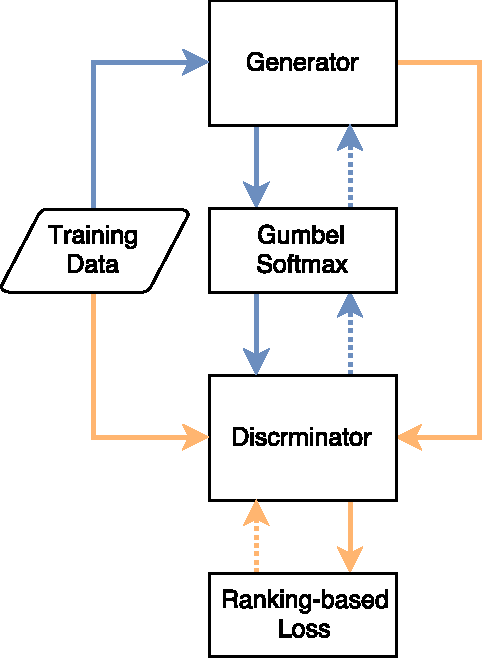
\includegraphics[width=0.35\textwidth]{overview.pdf}
    \caption{Overview of our training method. The solid lines indicate data input and dash lines show the direction of back propagation of gradients. Orange lines illustrate the process in which the discrminator uses generated negative samples and maximize the ranking-based objective. Blue lines shows the generator use discrminator as its feedback and propagate the gradient through gumbel softmax~\cite{GumbelSoftmax_Jiang_2016}.}
\label{system-overview}
\end{figure}

\subsection{Pretraining and bagging}

GANs are notoriously hard to train. To overcome this plight, Salimans et al.~\cite{}




% --------------------------------------
% related work

\section{Related work}

We continue to discuss the related work and make comparisons with our work in this section.

It's usually easier for generative models to do semi-supervised learning and anomaly detection. With the revival of neural networks and deep learning, the GAN~\cite{GAN} exploits the high fitting power of neural networks to train a generator alternatively with a discriminator model. 

TransG use translation assumption, and needs explicit density computation which is not that possible.
GAN can approach true distribution, blablabla.

% --------------------------------------
% experiments

\section{Experiments}

% --------------------------------------
% conclusion

\section{Conclusion}

% --------------------------------------
\section*{References}

\bibliography{adv-kb2e-bibfile}

\end{document}

% ====================================================
% reference snippets

% \paragraph{Installation} If the document class \emph{elsarticle} is not available on your computer, you can download and install the system package \emph{texlive-publishers} (Linux) or install the \LaTeX\ package \emph{elsarticle} using the package manager of your \TeX\ installation, which is typically \TeX\ Live or Mik\TeX.

% \paragraph{Usage} Once the package is properly installed, you can use the document class \emph{elsarticle} to create a manuscript. Please make sure that your manuscript follows the guidelines in the Guide for Authors of the relevant journal. It is not necessary to typeset your manuscript in exactly the same way as an article, unless you are submitting to a camera-ready copy (CRC) journal.

% \paragraph{Functionality} The Elsevier article class is based on the standard article class and supports almost all of the functionality of that class. In addition, it features commands and options to format the
% \begin{itemize}
% \item document style
% \item baselineskip
% \item front matter
% \item keywords and MSC codes
% \item theorems, definitions and proofs
% \item lables of enumerations
% \item citation style and labeling.
% \end{itemize}

% The author names and affiliations could be formatted in two ways:
% \begin{enumerate}[(1)]
% \item Group the authors per affiliation.
% \item Use footnotes to indicate the affiliations.
% \end{enumerate}
% See the front matter of this document for examples. You are recommended to conform your choice to the journal you are submitting to.